\documentclass{beamer}
\usetheme{default}

\usepackage{graphicx}
\graphicspath{{../../images/}}

\setbeamertemplate{caption}[numbered]

\title{Chapter-7: Pipeline / Pipe-and-Filter Architecture}
\subtitle{IF231303-Software Architecture\\Pradita University}
\author{Rizky wahyudi, Tommy Chitiawan, Mandalan}
\begin{document}
	\begin{frame}[plain]
		\maketitle
	\end{frame}

	\begin{frame}{Definisi}
		\begin{itemize}
	\item  Pipa dan Filter adalah pola arsitektur lain, yang memiliki entitas independen yang disebut filter (komponen) yang melakukan transformasi pada data dan memproses masukan yang mereka terima, dan pipa , yang berfungsi sebagai penghubung aliran data yang sedang diubah, masing-masing terhubung ke komponen berikutnya di dalam pipa.
\end{itemize}
\end{frame}

	\begin{frame}{Pipe and Filer Architecture Schema}
		\begin{figure}[h]
		\centering
		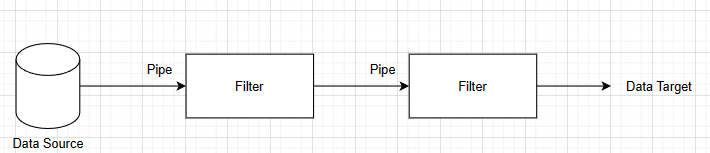
\includegraphics{Capture.png}
	\end{figure}
\end{frame}

\begin{frame}{kelebihan}
	\begin{itemize}
	\item Memastikan sambungan komponen, filter yang longgar dan fleksibel.
	\item Kopling longgar memungkinkan filter diubah tanpa modifikasi ke filter lain.
	\item Konduktif untuk pemrosesan paralel.
	\item Filter dapat diperlakukan sebagai kotak hitam. Pengguna sistem tidak perlu mengetahui logika di balik kerja setiap filter.
	\item Dapat digunakan kembali. Setiap filter dapat dipanggil dan digunakan berulang kali.
\end{itemize}
\end{frame}

\begin{frame}{kekurangan}
	\begin{itemize}
	\item 	Penambahan sejumlah besar filter independen dapat mengurangi kinerja karena overhead komputasi yang berlebihan.
	\item Bukan pilihan yang baik untuk sistem interaktif.
	\item Sistem pipa-dan-pemasang mungkin tidak cocok untuk perhitungan jangka panjang.
\end{itemize}

\end{frame}
		\begin{frame}{penerapan dalam aplikasi}
			\begin{itemize}
			\item Sistem pengolahan data: Pipe and filter dapat digunakan untuk mengambil data dari berbagai sumber dan memprosesnya melalui serangkaian filter untuk menghasilkan output yang diinginkan.
			
			\item Sistem pengolahan gambar: Pipe and filter dapat digunakan untuk memproses gambar atau video yang diambil dari kamera dengan menggunakan berbagai filter untuk menghasilkan gambar yang lebih baik atau memberikan efek khusus.
			
			\item Sistem pencarian: Pipe and filter dapat digunakan untuk memproses data pencarian yang diberikan oleh pengguna dan memfilter data untuk menghasilkan hasil pencarian yang relevan.
			
			\item Sistem pemrosesan audio: Pipe and filter dapat digunakan untuk memproses audio dan melakukan pengolahan suara seperti pengurangan kebisingan, pengaturan volume, dan pemotongan audio.
			
			\item Sistem pemrosesan teks: Pipe and filter dapat digunakan untuk memproses teks dan melakukan pengolahan bahasa alami seperti analisis sentimen dan pengenalan entitas.
		\end{itemize}
		\end{frame}
	\end{document}
	
		
		